%% This classfile tries to implement the lay-out of the beamer style beamerthemekuleuven2. This .sty-file can be downloaded here: https://www.kuleuven.be/communicatie/marketing/templates/presentatiemateriaal/index.html Not all options of the style are implemented in this class, for its purpose is merely to mimic the lay-out, and to provide a way to change the lay-out of presentations that were made using the "old" kulakbeamer class. For new documents, we recommend using the .sty-file instead.

\documentclass
   [kulak] % options: kul or kulak (default), handout 
   {kulakbeamer}

\usepackage[dutch]{babel}
\usepackage[utf8]{inputenc}
\usepackage[T1]{fontenc}
\usepackage{pgf-pie}

\title[Smart City]{Smart City}
\subtitle{\scriptsize Probleemoplossen en Ontwerpen Deel 2}
\author[Groep 6]{Groep 6}%eventueel nog aanpassen met onze namen
\institute[Kulak]{KU Leuven Kulak}
\date{Academiejaar 2020 -- 2021}
\author{\scriptsize Groep 6
	\tiny - Jolien Barbier, Mathis Bossuyt, Dieter Demuynck, Sarah De Meester, Rani Jans, Aaron Vandenberghe}

%% Overview at begin of each section; delete if unwanted.

\AtBeginSection[]{
	\begin{frame}
	\frametitle{Overzicht} %Change to "Outline" for English presentation
	{
		\hypersetup{hidelinks} %disable link colors
		\hfill	{\large\parbox{.95\textwidth}{\tableofcontents[currentsection,hideothersubsections]}}
	}
\end{frame}}

\begin{document}


\begin{titleframe}
\titlepage
\end{titleframe}


\section*{Inleiding}

\begin{frame}
\frametitle{Inleiding}
\begin{itemize}
	
	\item Wat: Zelfrijdend autootje met principe Smart City 
	\item Gekozen optie: Richtingsaanwijzers

	\begin{block}{Definitie: Smart City}
		Een stad waarbij informatietechnologie gebruikt wordt om de stad te beheren en te besturen. \cite{SmartCity}
	\end{block}
\end{itemize}
\end{frame}

\begin{frame}
\frametitle{Maatschappelijke relevantie autonome wagens}
\begin{itemize}
	\item Meer veiligheid
	\begin{itemize}
		\item Snellere reactie dan mensen
		\item Vermijden van ongelukken
	\end{itemize}
	\item Oplossing mobiliteitsproblemen
	\begin{itemize}
		\item Minder files
	\end{itemize}
	\item Milieubewust autotransport
	\begin{itemize}
		\item Kortste weg wordt gekozen
	\end{itemize}

\end{itemize}
\end{frame}

%\begin{outlineframe}[Overzicht]
%	\tableofcontents
%\end{outlineframe}

\section[Opdracht]{Opdracht}% eventueel aanpassen

\begin{frame}
\frametitle{De V's van vereisten}
\begin{columns}
	\column{.5\textwidth}
	\begin{itemize}
		\item \textbf{V}olglijnalgoritme
		\item \textbf{V}erkeerslichtinterpretatie (bijhorend bij stoplijn)
		\item \textbf{V}oorliggerdetectie

	\end{itemize}
	Extra's
	\begin{itemize}
		\item Acceptabele snelheid
		\item Manuele override
	\end{itemize}
	
	\column{.5\textwidth}
		\begin{figure}
			\centering
			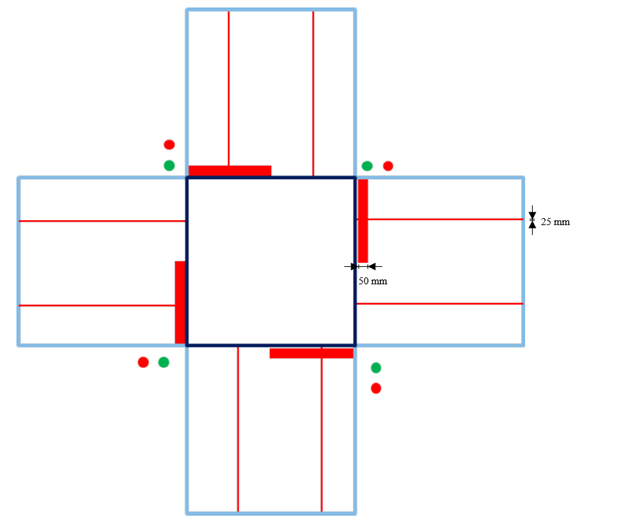
\includegraphics[width=.95\textwidth]{volglijnenEnStoplijnen}
			\caption{Kruispunt met volglijnen (25mm) en stoplijnen (50mm))}\cite{OpgavePO2}
		\end{figure}
	
\end{columns}

\end{frame}



\section{Aanpak}


%\subsection{Planning}
%\begin{frame}
%	\frametitle{Planning}
%	\begin{itemize}
%		\item Onderdelen vergelijken
%		\begin{itemize}
%			\item Budget in rekening houden
%			\item Stuklijst
%		\end{itemize}
%		\item Technisch
%		\begin{itemize}
%			\item 3D-modellen
%			\item Technische tekeningen
%		\end{itemize}
%		\item Praktisch
%		\begin{itemize}
%			\item Assemblage
%			\item Testen
%			\item Implementatie
%		\end{itemize}
%	\end{itemize}
%	
%\end{frame}

\subsection{Volledige wagen}
\begin{frame}
	\frametitle{Volledige wagen}
	\begin{figure}
		\centering
		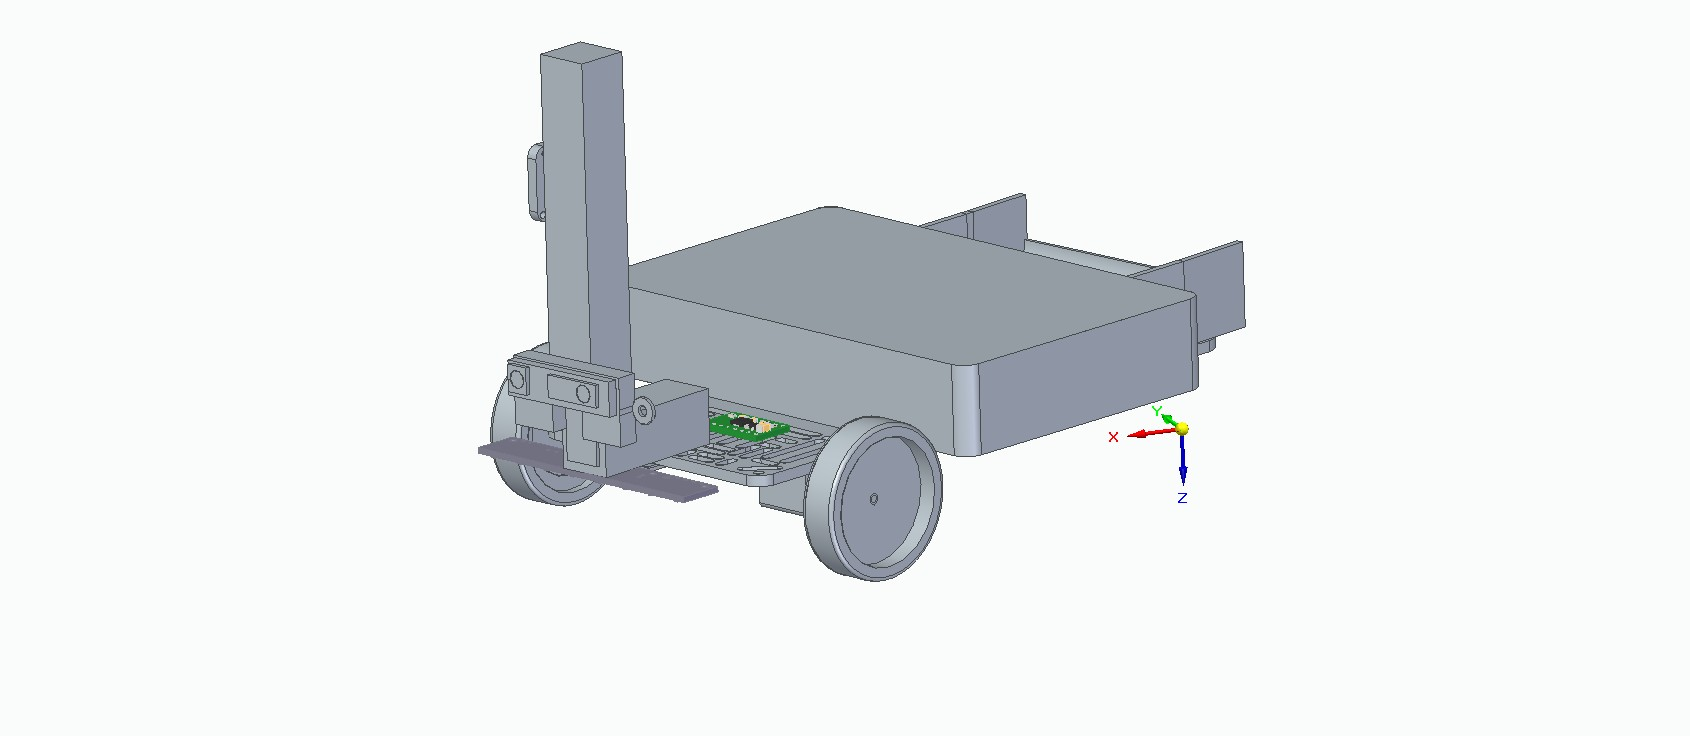
\includegraphics[width=.95\textwidth]{assemblageAuto}
		\caption{Assemblage van de wagen}
	\end{figure}
\end{frame}

\subsection{Onderdelen}

\begin{frame}
	\frametitle{Bodem} %chassis + wielen + motoren
	
	\begin{columns}
		\column{.25\textwidth}
		\begin{figure}
			\centering
			
\includegraphics[width=.45\textwidth]{chassis}
			\caption{\scriptsize Chassis}\cite{RobotChassisRechthoekigZwart}
		\end{figure}
		\column{.25\textwidth}
		\begin{figure}
			\centering
			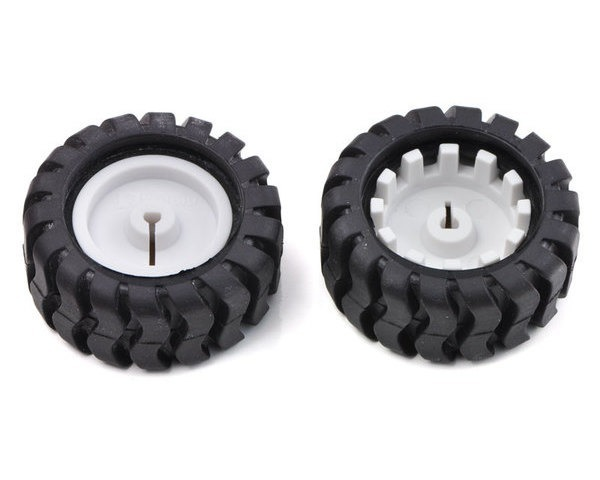
\includegraphics[width=.7\textwidth]{wielen}
			\caption{\scriptsize Wiel 42x19mm}\cite{Wiel42x19mm}
		\end{figure}
		\column{.25\textwidth}
		\begin{figure}
			\centering
			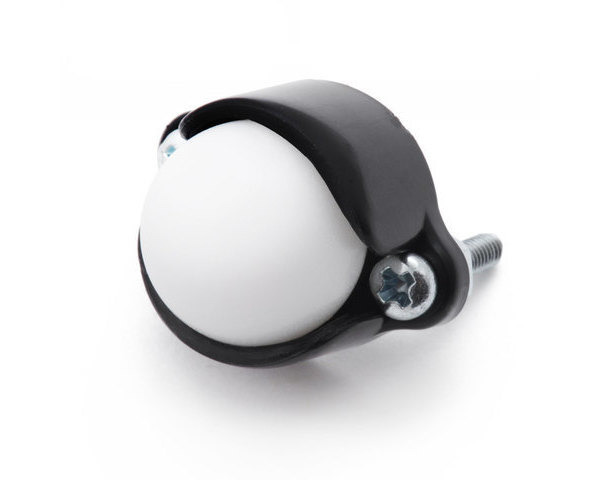
\includegraphics[width=.7\textwidth]{ballcaster}
			\caption{\scriptsize Ball Caster}\cite{BallCaster}
		\end{figure}
		\column{.25\textwidth}
		\begin{figure}
			\centering
			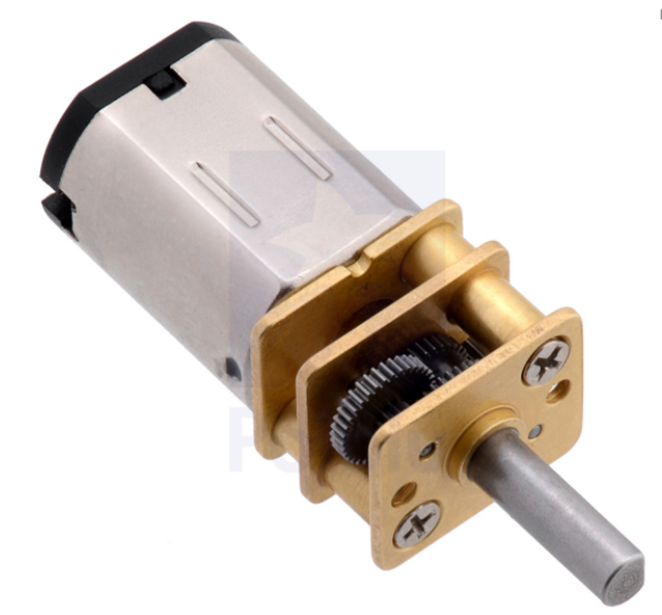
\includegraphics[width=.6\textwidth]{gear}
			\caption{\scriptsize Micro Metal Gear Motor 50:1 HP}\cite{MicroMetalGearMotor50:1HP}
		\end{figure}
	\end{columns}
	
\end{frame}
\begin{frame}
	\frametitle{Sensoren}
	Sensoren laten ons toe om informatie uit de buitenwereld te lezen
	\begin{columns}
		\column{.3\textwidth}
		\begin{figure}
			\centering
			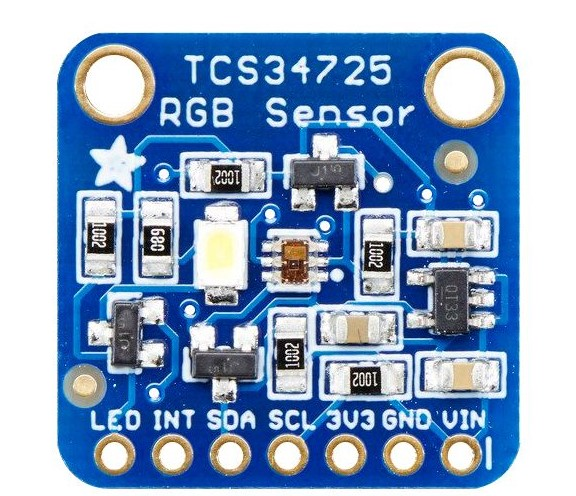
\includegraphics[width=.7\textwidth]{kleurensensor}
			\caption{Kleurensensor}\cite{TCS34725KleurSensorBOB}
		\end{figure}
		\column{.3\textwidth}
		\begin{figure}
			\centering
			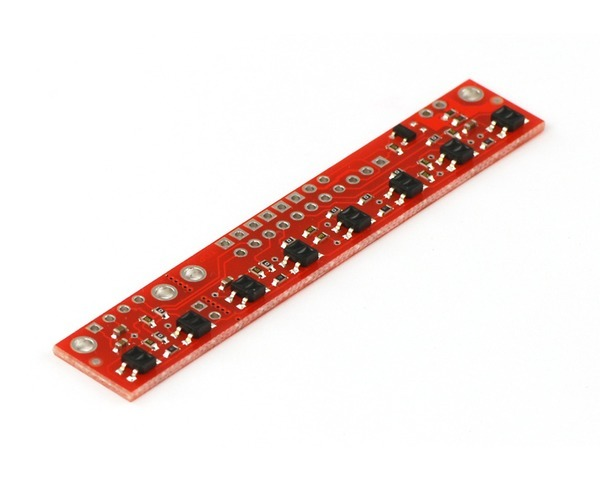
\includegraphics[width=.8\textwidth]{reflectiesensor}
			\caption{Analoge reflectiesensor}\cite{QTR-8AAnalogeReflexieSensorArray}
		\end{figure}
		\column{.3\textwidth}
		\begin{figure}
			\centering
			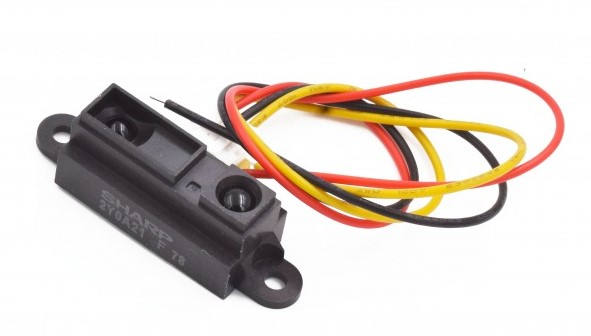
\includegraphics[width=.9\textwidth]{afstandssensor}
			\caption{Analoge afstandssensor}\cite{AnalogeAfstandssensor}
		\end{figure}
	\end{columns}
	
\end{frame}



\begin{frame}
	\frametitle{Microcontroller}
	De microcontroller maakt het mogelijk om binnengekregen signalen van sensoren te verwerken
	\begin{columns}
		\column{.5\textwidth}
		\begin{figure}
			\centering
			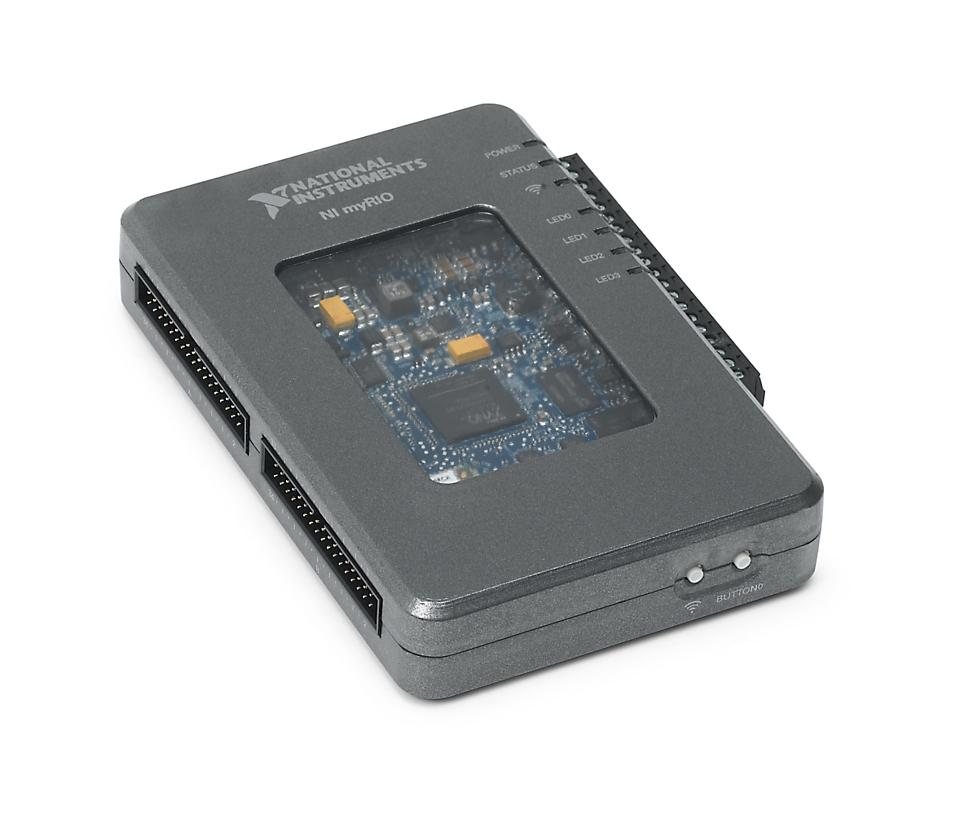
\includegraphics[width=.7\textwidth]{NI-myrio}
			\caption{NI MyRio}\cite{nimyrio}
		\end{figure}
		\column{.5\textwidth}
		%\begin{figure}
		%	\centering
		%	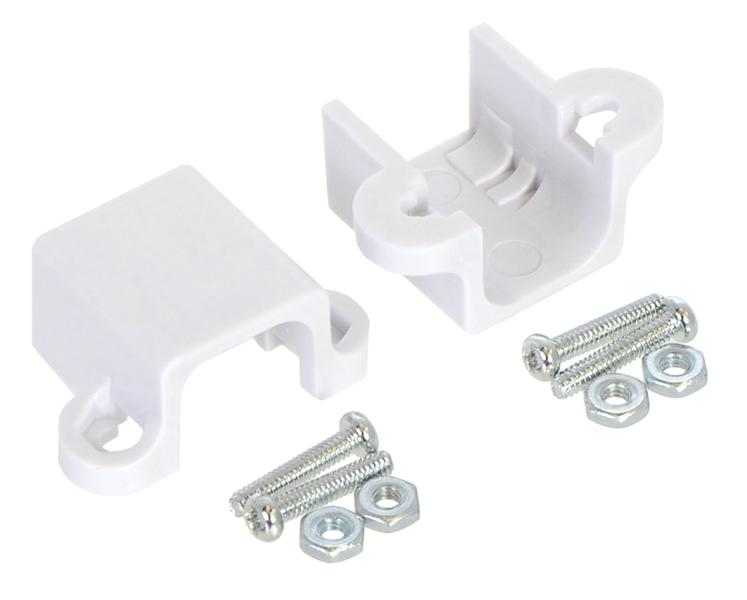
\includegraphics[width=.7\textwidth]{beugel}
		%	\caption{Motorbeugel}\cite{MicroMetalGearMotorBeugel}
		%\end{figure}
	\end{columns}
	
\end{frame}


\subsection{Prijsbesteding}
\begin{frame}
	\frametitle{Prijsbesteding}
	\begin{itemize}
		\item Budget: 3500 eenheden
	\end{itemize}
	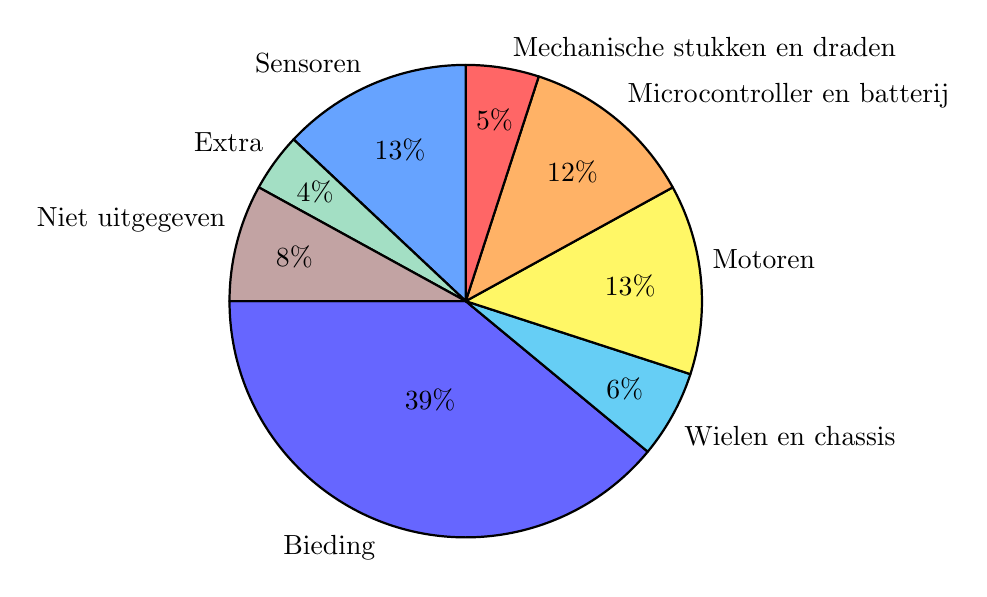
\begin{tikzpicture}
		\pie [rotate = 180]
		{39/ Bieding, 6/ Wielen en chassis, 13/ Motoren, 12/ Microcontroller en batterij, 5/ Mechanische stukken en draden, 13/ Sensoren, 4/ Extra, 8/ Niet uitgegeven}
	\end{tikzpicture}
\end{frame}



\section[Experimenten]{Experimenten met LabVIEW}

\begin{frame}
	\frametitle{Experimenten}
	\begin{itemize}
		\item Voorbeeldprogramma's voor sensoren
		\item Testen
		\begin{itemize}
			\item Reflectiesensor: witte bladzijde en zwart omhulsel laptop
			\item Afstandssensor: afstand object variëren
			\item nog aan te vullen
		\end{itemize}
	\end{itemize}.
\end{frame}



\section{Besluit}
\begin{frame}
\frametitle{Besluit}

\end{frame}


\begin{frame}
\frametitle{Mogelijke vragen}
	\begin{itemize}
		\item 
		\item 
		\item 
		\item 
	\end{itemize}
\end{frame}

\begin{frame}
\frametitle{Bronvermelding}
	\bibliographystyle{plain}
	\bibliography{bronnen_verslag}
	\bibliographystyle{unsrt}
\end{frame}

\end{document}
